%---------------------------------------------------------------------------%
%-                                                                         -%
%-                           LaTeX Template                                -%
%-                                                                         -%
%---------------------------------------------------------------------------%
%- Copyright (C) Huangrui Mo <huangrui.mo@gmail.com> 
%- This is free software: you can redistribute it and/or modify it
%- under the terms of the GNU General Public License as published by
%- the Free Software Foundation, either version 3 of the License, or
%- (at your option) any later version.
%---------------------------------------------------------------------------%
%->> Document class declaration
%---------------------------------------------------------------------------%
\documentclass{Style/ucasproposal}%
%- Multiple optional arguments:
%- [<oneside|twoside|print>]% oneside eprint, twoside eprint, or paper print
%- [fontset=<adobe|none|...>]% specify font set instead of automatic detection
%- [scheme=plain]% thesis writing of international students
%- [draftversion]% show draft version information
%- [standard options for ctex article class: draft|paper size|font size|...]%
%---------------------------------------------------------------------------%
%->> Document settings
%---------------------------------------------------------------------------%
\usepackage[numbers,list,xhf]{Style/artratex}% document settings
%- usage: \usepackage[option1,option2,...,optionN]{artratex}
%- Multiple optional arguments:
%- [bibtex|biber]% set bibliography processor and package
%- [<numbers|super|authoryear|alpha>]% set citation and reference style
%- <numbers>: textual: Jones [1]; parenthetical: [1]
%- <super>: textual: Jones superscript [1]; parenthetical: superscript [1]
%- <authoryear>: textual: Jones (1995); parenthetical: (Jones, 1995)
%- <alpha>: textual: not available; parenthetical: [Jon95]
%- [geometry]% reconfigure page layout via geometry package
%- [lscape]% provide landscape layout environment
%- [xhf]% disable header and footer via fancyhdr package
%- [color]% provide color support via xcolor package
%- [background]% enable page background
%- [tikz]% provide complex diagrams via tikz package
%- [table]% provide complex tables via ctable package
%- [list]% provide enhanced list environments for algorithm and coding
%- [math]% enable some extra math packages
%- [xlink]% disable link colors
\usepackage{Style/artracom}% user defined commands
%---------------------------------------------------------------------------%
%->> Document inclusion
%---------------------------------------------------------------------------%
%\includeonly{Tex/Chap_1,...,Tex/Chap_N}% selected files compilation
%---------------------------------------------------------------------------%
%->> Document content
%---------------------------------------------------------------------------%
%-
%-> Titlepage information
%-
%-> 中文封面信息
%-
\schoollogo{scale=0.112}{ucas_logo}% 校徽
\title{多架构软硬协同二进制翻译的实现和优化}% 题目
\author{晏悦}% 作者姓名
\authorid{202128013229037}% 学号
\advisor{王剑}% 指导老师
\advisortitle{研究员}% 指导老师职务
\degree{硕士}% 学位:硕士、博士
\degreetype{工学}% 学位类别:理学、工学、工程、医学等
\major{计算机系统结构}% 二级学科专业名称
\field{体系结构}% 研究方向
\institute{中国科学院计算技术研究所}% 院所
%\institute{中国科学院力学研究所\\流固耦合实验室}% 多行院所名称示例
%\chinesedate{2014~年~06~月}% 日期
%---------------------------------------------------------------------------%
\begin{document}
%-
%-> Frontmatter: title page, abstract, content list, symbol list, preface
%-
\pagenumbering{roman}% page numbers with roman style
% \input{Tex/Frontmatter}% title page, abstract

%---------------------------------------------------------------------------%
%-> Frontmatter
%---------------------------------------------------------------------------%
%-
%-> 生成封面
%-
\maketitle% 生成中文封面
%-
%-> 目录
%-
\tableofcontents% 生成目录
%---------------------------------------------------------------------------%
%-
%-> Mainmatter
%-
\clearpage
\pagenumbering{arabic}% restart page numbers with arabic style
% %---------------------------------------------------------------------------%
%->> Main content
%---------------------------------------------------------------------------%
\section{选题的背景及意义}

\subsection{选题背景}

关于riscv生态,以及各类指令集生态的问题。

阐述二进制翻译器的问题,以及二进制翻译器的优势。



\subsubsection{背景}


\subsection{选题意义}



\subsubsection{意义}



\section{国内外本学科领域的发展现状与趋势}



\section{课题主要研究内容、预期目标}



\section{拟采用的研究方法、技术路线、实验方案及其可行性分析}



\section{已有科研基础与所需的科研条件}



\section{研究工作计划与进度安排}



\section*{填表说明}

本表内容须真实、完整、准确。

\section*{常见使用问题}

\begin{enumerate}
    \item 模板使用说明请见 \href{https://github.com/mohuangrui/ucasthesis}{ucasthesis:中国科学院大学学位论文 LaTeX 模板}.
    \item 填表说明和模板说明不是开题报告的一部分,请删除。
    \item 开题报告样式设计导致对题目换行与不换行难以兼容,排版十分困难。推荐采用当前设置,尽量避免将精力花在这些无关紧要的细节上。
\end{enumerate}

\nocite{*}% 使文献列表显示所有参考文献(包括未引用文献)
%---------------------------------------------------------------------------%
% main content
%---------------------------------------------------------------------------%
%->> Main content
%---------------------------------------------------------------------------%
\section{选题的背景及意义}

随着计算机技术的发展,各种指令集架构层出不穷,如X86、ARM、LoongArch\cite{LoongArch2023}、RISCV等。这些指令集之间互不兼容,导致软件需要针对不同架构进行多次开发和编译,无法进行通用迁移,增加了软件开发的成本和复杂度。

\subsection{中国国产CPU的多样性}

% https://zhuanlan.zhihu.com/p/599483286 国产CPU的发展现状
中国国产CPU在多个架构上展现出丰富多彩的发展,其中X86、ARM、LoongArch和RISCV等架构代表了不同的技术路线,由各个公司推动。参见表\ref{tab:CPUs},以下是各架构的特点:

% https://www.tablesgenerator.com/latex_tables 生成latex表格
\begin{table}[]
\centering
\caption{国产CPU的发展现状}
\label{tab:CPUs}
    \begin{tabular}{llll}
    \rowcolor[HTML]{FBE5D6} 
    指令集       & 代表公司   & 优势        & 不足         \\
    X86       & 兆芯,海光  & 兼容Windows & 授权问题,AVX专利 \\
    ARM       & 华为,飞腾  & 兼容安卓      & 授权问题       \\
    LoongArch & 龙芯     & 自主可控      & 生态不足       \\
    RISCV     & 开芯院,阿里 & 开源开放      & 生态不足      
    \end{tabular}
    \end{table}


    \begin{itemize}
    \item {X86架构: } 代表公司为兆芯和海光,采用X86架构IP内核授权模式,可基于公版CPU核进行优化或修改,性能起点高,生态壁垒相对低。但是依赖海外企业授权,自主可控风险偏高。
    
    \item{ARM架构:} 代表公司为华为和飞腾,采用Armv8永久授权,具有更高的自主化程度,可自行研发设计CPU内核和芯片,也可扩充指令集。但是存在长期隐患,因为Arm将不再向这些国产CPU厂商提供Armv9的永久授权。
    
    \item{LoongArch架构:} 代表公司为龙芯,采用LoongArch指令集,具有相对更高的自主可控程度,已经在国产军工行业得到了广泛应用。但是生态不足,需要大量投入才能建立起完善的软件生态。
    
    \item{RISCV架构:} 代表公司为开源芯片研究院和阿里平头哥,采用RISCV架构,具有相对精简的指令集架构(ISA),并遵循开源宽松的BSD协议,在国内得到了迅速发展,但同样生态不足。
    \end{itemize}


\subsection{指令集生态的碎片化与兼容性问题}

\begin{figure}[h]
    \centering
    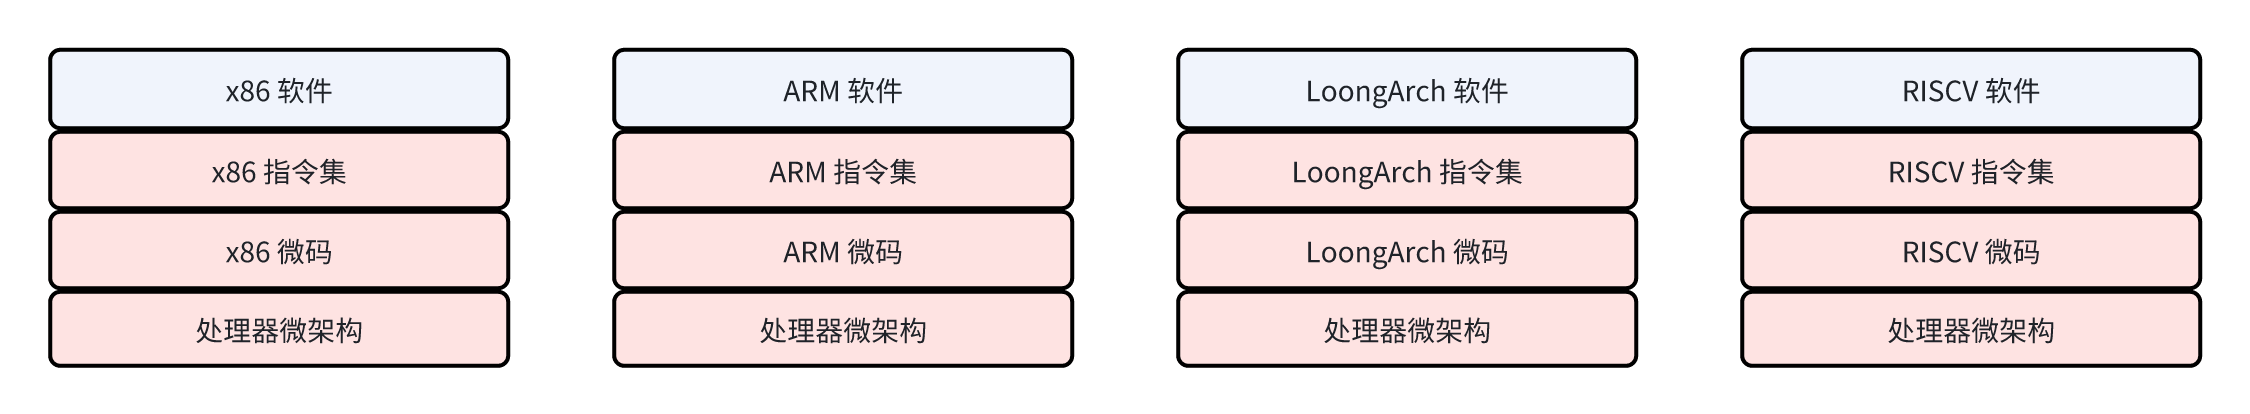
\includegraphics[width=1\linewidth]{./feishuImage/allCPU_arch.png}
    \caption{不同指令集CPU的架构图,图中白色为软件层,红色为硬件层,并忽略了操作系统,这不是本文研究重点。\protect\footnotemark}
    \label{img:allCPU_arch}
  \end{figure}

\footnotetext{ARM, LoongArch, RISCV 等精简指令集架构(RISC)的CPU,内部可以实现微码层,也可以不实现,根据具体CPU微架构实现而不同。}

如图\ref{img:allCPU_arch}所示,同一套软件源代码需要针对不同的指令集进行编译才能在不同架构的CPU上运行。

    而中国国产CPU的多样性导致了指令集的碎片化,增加了应用程序在不同架构间迁移和适配的复杂性。存在的问题包括:
    \begin{itemize}
    \item 适配和迁移负担: 不同架构间的适配和迁移需要大量人力和物力资源。
    
    \item 历史兼容包袱: 不同指令集的历史兼容包袱使得跨架构的兼容性复杂。
    
    \item 编译与源代码的限制: 古老软件无源代码,只能通过翻译运行以适应新的指令集。
    
    \item 操作系统支持的挑战: 操作系统厂商需要投入更多资源以支持不同架构。
    \end{itemize}

\subsection{二进制翻译技术的重要性}
目前,二进制翻译技术是解决指令集兼容性问题的主要方法。

\begin{figure}[h]
    \centering
    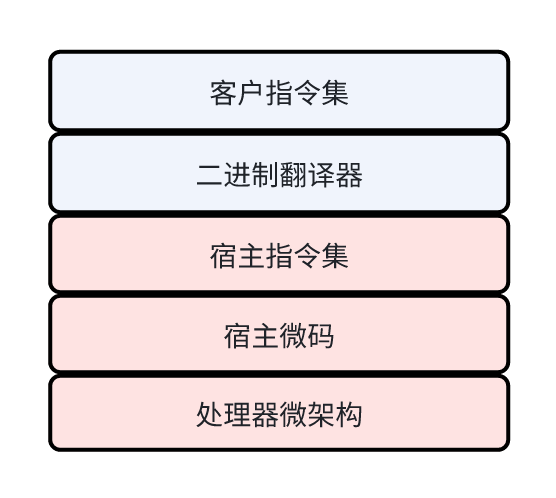
\includegraphics[width=0.3\linewidth]{./feishuImage/BT_arch.png}
    \caption{二进制翻译器架构图,能在宿主指令集机器上运行客户程序。}
    \label{img:BT_arch}
  \end{figure}

如图\ref{img:BT_arch} 二进制翻译技术能够将一个指令集(称为客户指令集)上的二进制程序翻译到另一种指令集(称为宿主指令集)上执行,分为系统级和用户级二进制翻译。系统级翻译涉及整个操作系统,而用户级翻译主要处理用户程序。用户级翻译由于不需要模拟特权态和物理内存,因此性能更高,在软件生态迁移中更为常见,在后文中提及的二进制翻译器默认为用户级二进制翻译器。

\subsection{二进制翻译器性能问题}
现有的开源二进制翻译器性能
\footnote{
    目前工业界和学术界对二进制翻译的性能有着默认统一的定义:同一份测试程序的源码用相同编译参数,编译到客户指令集和宿主指令集,得到两份二进制文件$B_g$和$B_h$。
    在硬件平台用二进制翻译运行客户程序$B_g$的时间记为$T_{bt}$,在同一硬件平台直接运行宿主程序$B_h$的时间记为$T_h$。
    二进制翻译的性能则为两个运行时间的比值$\frac{T_h}{T_{bt}}$。
}
相对较低,例如QEMU\cite{bellardQEMUFastPortable2005}虽然支持多架构应用,但在翻译运行SPECCPU 2017\cite{SPECCPU2017}程序时候,仅有约10\%的性能。商业二进制翻译器也存在性能损失,
如苹果的Rosetta2\cite{RosettaTranslationEnvironment, RunningIntelBinaries}、
华为的ExaGear\cite{KunPengExaGear}、
和龙芯的LATX\cite{LoongArchEnv2022, LoongArch2023},
性能仅达到原生运行的70\%左右,并且仅能保证单一指令集翻译到单一指令集,并不通用,多架构支持较为困难。这直接影响了软件生态迁移的流畅度和成功性。

\subsection{多架构软硬协同二进制翻译的需求}

为了解决指令集碎片化和二进制翻译器性能问题,迫切需要多架构软硬协同的二进制翻译技术。这项技术的关键目标是在同一套硬件下实现多指令集的共存,为软件提供更好的跨平台兼容性和性能表现。

这种技术的优势在于:

1. \textbf{打破指令集边界,消除应用迁移成本:} 应用程序无需适配和迁移至特定指令集,可直接在同一套硬件上运行,降低了软件开发和维护的复杂性。

2. \textbf{硬件对外暴露微码,规避X86等授权问题:} 通过在硬件层面暴露微码,技术在一定程度上规避了X86等架构的授权问题,提高了国产CPU的自主性。

3. \textbf{软件维护历史兼容,微码迭代优化:} 作为软件层面的核心组件,二进制翻译器维护历史兼容性并实现微码迭代优化,确保不同架构的硬件在不同历史时期的应用中保持高效运行。

如图\ref{img:my_arch}所示,本文提出了一种多架构软硬协同的二进制翻译技术,通过在硬件层面支持一套融合微码,为软件层面的二进制翻译器提供更好的性能和兼容性。这项技术可降低软件开发和维护的复杂性,弥合不同指令集的生态差异,对中国国产CPU的发展具有重要意义。


\begin{figure}[h]
    \centering
    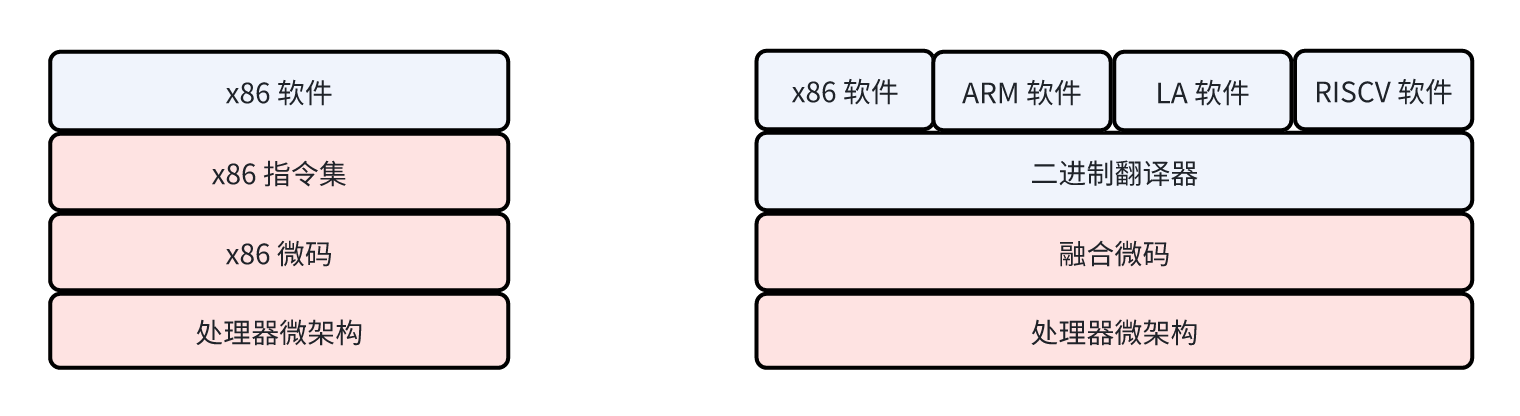
\includegraphics[width=1\linewidth]{./feishuImage/my_arch.png}
    \caption{多架构软硬协同的二进制翻译架构图,硬件仅对外暴露微码,软件层面的二进制翻译器可以实现多架构的支持。}
    \label{img:my_arch}
  \end{figure}


\section{国内外本学科领域的发展现状与趋势}



\section{课题主要研究内容、预期目标}



\section{拟采用的研究方法、技术路线、实验方案及其可行性分析}



\section{已有科研基础与所需的科研条件}



\section{研究工作计划与进度安排}


% \nocite{*}% 使文献列表显示所有参考文献(包括未引用文献)
%---------------------------------------------------------------------------%



%-
%-> Backmatter: bibliography, glossary, index
%-
\artxifstreq{\artxbib}{bibtex}{% enable bibtex
    \bibliography{./kaiti.bib}% bibliography
}{%
    \printbibliography% bibliography
}
\end{document}
%---------------------------------------------------------------------------%

